\documentclass[a4]{article}
\pagestyle{myheadings}

%%%%%%%%%%%%%%%%%%%
% Packages/Macros %
%%%%%%%%%%%%%%%%%%%
\usepackage{mathrsfs}


\usepackage{fancyhdr}
\pagestyle{fancy}
\lhead{}
\chead{}
\rhead{}
\lfoot{}
\cfoot{} 
\rfoot{\normalsize\thepage}
\renewcommand{\headrulewidth}{0pt}
\renewcommand{\footrulewidth}{0pt}
\newcommand{\RomanNumeralCaps}[1]
    {\MakeUppercase{\romannumeral #1}}

\usepackage{amssymb,latexsym}  % Standard packages
\usepackage[utf8]{inputenc}
\usepackage[russian]{babel}
\usepackage{MnSymbol}
\usepackage{mathrsfs}
\usepackage{amsmath,amsthm}
\usepackage{indentfirst}
\usepackage{graphicx}%,vmargin}
\usepackage{graphicx}
\graphicspath{{pictures/}} 
\usepackage{verbatim}
\usepackage{color}
\usepackage[nottoc,numbib]{tocbibind}
\usepackage{float}

\usepackage{listings}
\definecolor{codegreen}{rgb}{0,0.6,0}
\definecolor{codegray}{rgb}{0.5,0.5,0.5}
\definecolor{codepurple}{rgb}{0.58,0,0.82}
\definecolor{backcolour}{rgb}{0.95,0.95,0.92}
 
\lstdefinestyle{mystyle}{
    backgroundcolor=\color{backcolour},   
    commentstyle=\color{codegreen},
    keywordstyle=\color{magenta},
    numberstyle=\tiny\color{codegray},
    stringstyle=\color{codepurple},
    basicstyle=\footnotesize,
    breakatwhitespace=false,         
    breaklines=true,                 
    captionpos=b,                    
    keepspaces=true,                 
    numbers=left,                    
    numbersep=5pt,                  
    showspaces=false,                
    showstringspaces=false,
    showtabs=false,                  
    tabsize=2
}
 
\lstset{style=mystyle}

\usepackage{url}
\urldef\myurl\url{foo%.com}





\DeclareGraphicsExtensions{.pdf,.png,.jpg}% -- настройка картинок

\usepackage{epigraph} %%% to make inspirational quotes.
\usepackage[all]{xy} %for XyPic'a
\usepackage{color} 
\usepackage{amscd} %для коммутативных диграмм
%\usepackage[colorlinks,urlcolor=red]{hyperref}

%\renewcommand{\baselinestretch}{1.5}
%\sloppy
%\usepackage{listings}
%\lstset{numbers=left}
%\setmarginsrb{2cm}{1.5cm}{1cm}{1.5cm}{0pt}{0mm}{0pt}{13mm}


\newtheorem{Lemma}{Лемма}[section]
\newtheorem{Proposition}{Предложение}[section]
\newtheorem{Theorem}{Теорема}[section]
\newtheorem{Corollary}{Следствие}[section]
\newtheorem{Remark}{Замечание}[section]
\newtheorem{Definition}{Определение}[section]
\newtheorem{Designations}{Обозначение}[section]




%%%%%%%%%%%%%%%%%%%%%%% 
%Подготовка оглавления% 
%%%%%%%%%%%%%%%%%%%%%%% 
\usepackage[titles]{tocloft}
\renewcommand{\cftdotsep}{2} %частота точек
\renewcommand\cftsecleader{\cftdotfill{\cftdotsep}}
\renewcommand{\cfttoctitlefont}{\hspace{0.38\textwidth} \LARGE\bfseries} 
\renewcommand{\cftsecaftersnum}{.}
\renewcommand{\cftsubsecaftersnum}{.}
\renewcommand{\cftbeforetoctitleskip}{-1em} 
\renewcommand{\cftaftertoctitle}{\mbox{}\hfill \\ \mbox{}\hfill{\footnotesize Стр.}\vspace{-0.5em}} 
%\renewcommand{\cftchapfont}{\normalsize\bfseries \MakeUppercase{\chaptername} } 
%\renewcommand{\cftsecfont}{\hspace{1pt}} 
\renewcommand{\cftsubsecfont}{\hspace{1pt}} 
%\renewcommand{\cftbeforechapskip}{1em} 
\renewcommand{\cftparskip}{3mm} %определяет величину отступа в оглавлении
\setcounter{tocdepth}{5} 
\renewcommand{\listoffigures}{\begingroup %добавляем номер в список иллюстраций
\tocsection
\tocfile{\listfigurename}{lof}
\endgroup}
\renewcommand{\listoftables}{\begingroup %добавляем номер в список иллюстраций
\tocsection
\tocfile{\listtablename}{lot}
\endgroup}


   
   
%\renewcommand{\thelikesection}{(\roman{likesection})}
%%%%%%%%%%%
% Margins %
%%%%%%%%%%%
\addtolength{\textwidth}{0.7in}
\textheight=630pt
\addtolength{\evensidemargin}{-0.4in}
\addtolength{\oddsidemargin}{-0.4in}
\addtolength{\topmargin}{-0.4in}

%%%%%%%%%%%%%%%%%%%%%%%%%%%%%%%%%%%
%%%%%%Переопределение chapter%%%%%% 
%%%%%%%%%%%%%%%%%%%%%%%%%%%%%%%%%%%
\newcommand{\empline}{\mbox{}\newline} 
\newcommand{\likechapterheading}[1]{ 
\begin{center} 
\textbf{\MakeUppercase{#1}} 
\end{center} 
\empline} 

%%%%%%%Запиливание переопределённого chapter в оглавление%%%%%% 
\makeatletter 
\renewcommand{\@dotsep}{2} 
\newcommand{\l@likechapter}[2]{{\bfseries\@dottedtocline{0}{0pt}{0pt}{#1}{#2}}} 
\makeatother 
\newcommand{\likechapter}[1]{ 
\likechapterheading{#1} 
\addcontentsline{toc}{likechapter}{\MakeUppercase{#1}}} 




\usepackage{xcolor}
\usepackage{hyperref}
\definecolor{linkcolor}{HTML}{000000} % цвет ссылок
\definecolor{urlcolor}{HTML}{AA1622} % цвет гиперссылок
 
\hypersetup{pdfstartview=FitH,  linkcolor=linkcolor,urlcolor=urlcolor, colorlinks=true}

%%%%%%%%%%%%
% Document %
%%%%%%%%%%%%

%%%%%%%%%%%%%%%%%%%%%%%%%%%%%
%%%%%%главы -- section*%%%%%%
%%%%section -- subsection%%%%
%subsection -- subsubsection%
%%%%%%%%%%%%%%%%%%%%%%%%%%%%%
\def \newstr {\medskip \par \noindent} 



\begin{document}
\def\contentsname{\LARGE{Содержание}}
\thispagestyle{empty}
\begin{center} 

\vspace{2cm} 
{\Large \sc Санкт-Петербургский Политехнический}\\
\vspace{2mm}
{\Large \sc Университет} им. {\Large\sc Петра Великого}\\
\vspace{1cm}
{\large \sc Институт прикладной математики и механики\\ 
\vspace{0.5mm}
\textsc{}}\\ 
\vspace{0.5mm}
{\large\sc Кафедра прикладной математики}\\
\vspace{15mm}


%\rule[0.5ex]{\linewidth}{2pt}\vspace*{-\baselineskip}\vspace*{3.2pt} 
%\rule[0.5ex]{\linewidth}{1pt}\\[\baselineskip] 
{\huge \sc Сводный отчет по лабораторным 1-4.

 }
\vspace*{2mm}
%\rule[0.7ex]{\linewidth}{1pt}\vspace*{-\baselineskip}\vspace{3.2pt} 
%\rule[0.5ex]{\linewidth}{2pt}\\ 


\vspace{1cm}

{\sc $3$ курс$,$ группа $3630102/70301$}

\vspace{2cm} 
Студент группы $3630102/70301$ \hfill Лебедев К.С.\\
\vspace{1cm}
Преподаватель \hfill Баженов А. Н.\\
\vspace{20mm} 

\end{center} 
%\author{Я}
\begin{center}
\vfill {\large\textsc{Санкт-Петербург}}\\ 
2020 г.
\end{center}

%%%%%%%%%%%%%%%%%%%%%%%%%%%%%%%%%%%%%%%%%%%%%%%%%%%%%%%%%%%%%%%%%%%%%%%%%%%%%%%%%%%%%%%%%%%%%%
%\ \\[4cm]

%\rm
%%%%%%%%%%%%%%%%%%%%%%%%%%%%%%%%%%%%%%%%%%%%%%%%%%%%%%%%%%%%%%%%%%%%%%%%%%%%%%%%%%%%%%%%%%%%%%
\newpage
\pagestyle{plain}

%\begin{center}
%\begin{abstract} 

%\end{abstract}

%\end{center}

\newpage
\tableofcontents{}
\newpage
\listoffigures{}
\newpage

\section{Постановка задачи}
Сгенерировать выборки различных размеров для $5$-ти распределений.
На основе этих выборок:
\begin{enumerate}
\item Построить гистограммы распределения
\item Вычислить характеристики положения ($\overline{x},\; med\; x,\; Z_R,\; Z_Q,\; Z_{tr},$ при $r = \frac{n}{4}.$)
\item Построить боксплот и исследовать распределение на выбросы
\item Построить эмпирические функции распределения и ядерные оценки
\end{enumerate}

\section{Теория}

\subsection{Плотности распределений}
\begin{enumerate}
\item Стандартное нормальное распределения \cite{distr_formulas}: 
	\begin{equation}\label{eqn:normal}
	N(x,0,1) = \frac{1}{\sqrt{2\pi}}e^{-\frac{x^2}{2}}
	\end{equation} 
\item Распределение Коши\cite{distr_formulas}: 
	\begin{equation}\label{eqn:cauchy}
	 C(x,0,1) = \frac{1}{\pi(1+x^2)}
	 \end{equation}
\item Распределение Лапласа\cite{distr_formulas}: 
	 \begin{equation}\label{eqn:laplace}
	 L\left( x,0,\frac{1}{\sqrt{2}}\right) = \frac{1}{\sqrt{2}}e^{-\sqrt{2}\vert x\vert}
	 \end{equation}
\item Распределение Пуассона\cite{distr_formulas}:
	 \begin{equation}\label{eqn:poisson}
	 P(\lambda,k) = \frac{\lambda^k}{k!}e^{-\lambda}
	\end{equation}  
\item Равномерное распределение\cite{distr_formulas}: 
	\begin{equation}\label{eqn:uniform}
	M(x,-\sqrt{3}, \sqrt{3}) = 
	 \begin{cases}
	   \frac{1}{2\sqrt{3}} &\vert x\vert \leqslant \sqrt{3}\\
	   0 &\vert x\vert > \sqrt{3}
	 \end{cases}
\end{equation}
\end{enumerate}

\subsection{Характеристики положения}
\begin{enumerate}
\item Выборочное среднее \cite{average}:
\begin{equation}\label{eqn:average}
\overline{x} = \frac{1}{n}\sum_{i=1}^n x_i \hfill  
\end{equation}
\item Выборочная медиана \cite{med}:
\begin{equation}
med\; x = \begin{cases}
x_{k+1}, & n = 2k+1\\
\frac{1}{2}\left(x_k+x_{k+1}\right), & n = 2k
\end{cases} \hfill  \label{eqn:med}
\end{equation}
\item Полусумма экстремальных значений \cite{mean_extr}:
\begin{equation}
Z_R = \frac{1}{2}\left(x_1+x_n\right) \hfill  \label{eqn:mean_extr}
\end{equation}
\item Полусумма квартилей \cite{quartiles}:
\begin{equation}
Z_Q = \frac{1}{2}\left(Z_{\frac{1}{4}}+Z_{\frac{3}{4}}\right) \hfill  \label{eqn:quartiles}
\end{equation}
\item Усечённое среднее \cite{cut_mean}:
\begin{equation}
Z_{tr} = \frac{1}{n - 2r}\sum_{i=r+1}^{n-r} x_i \hfill  \label{eqn:cut_mean}
\end{equation}
\end{enumerate}

\subsection{Боксплот Тьюки}

Боксплот Тьюки - график, использующийся в описательной статистике, изображающий одномерное распределение вероятностей.

Такой вид диаграммы в удобной форме показывает медиану, нижний и верхний квартили, минимальное и максимальное значение выборки и выбросы.

\begin{enumerate}
\item Выборочная медиана \cite{med}:
\begin{equation}
med\; x = \begin{cases}
x_{k+1}, & n = 2k+1\\
\frac{1}{2}\left(x_k+x_{k+1}\right), & n = 2k
\end{cases} \hfill  \label{eqn:med}
\end{equation}

\item Квартиль \cite{quart}:
\begin{equation}
z_{[p]} = \begin{cases}
x_{np}, & np \in \mathbb{Z}\\
x_{[np]+1}, & np \notin \mathbb{Z}
\end{cases} \hfill  \label{eqn:quart}
\end{equation}
\end{enumerate}

\subsection{Эмпирическая функция и ядерная оценка плотности}
Эмпирическая функция распределения \cite{emp}, построенная по выборке $X = \left(X_1,\ldots, X_n\right)$ есть случайная функция $F_n(y),$ определённая на $\mathbb{R}:$
\begin{equation}
F_n(y) = \sum\limits_{i=1}^n I\left(X_i < y\right) \;\;\text{где}\; I\left(X_i < y\right) = \begin{cases} 
1, & X_i < y\\
0, & \text{иначе}
\end{cases}\hfill\label{eqn:emp}
\end{equation}

$X = \left(X_1,\ldots, X_n\right)$ есть одномерная выборка одинаково распределённых элементов, с плотностью распределения $f.$

Ядерная оценка плотности \cite{art}:
\begin{equation}
    f_h(x) = \frac{1}{nh}\sum\limits_{i=1}^nK\left(\frac{x-x_i}{h}\right)\label{eqn:art}
\end{equation}
где $K$ является ядром, а $h>0$ является сглаживающим параметром, и называется шириной полосы.

В данной работе в качестве ядра была выбрана плотность вероятности стандартного нормального распределения \cite{link:pdf}:

\begin{equation}
    K(x) = \frac{1}{\sqrt{2\pi}}e^{-\frac{x^2}{2}}
\end{equation}
\section{Реализация}
Для генерации выборки был использован $Python\;3.6$: модуль $random$ библиотеки $numpy$ для генерации случайных чисел с различными распределениями и библиотека $matplotlib$ для построения графиков и гистограмм. Функции распределения обрабатывались при помощи библиотеки scipy.stats.

\section{Результаты}
\subsection{Стандартное нормальное распределение}
	\begin{figure}[H]
	\caption{Гистограмма нормального распределения}
	\includegraphics[width=\textwidth]{lab1/distribution_normal.png}
	\end{figure}
	\begin{figure}[H]
	\caption{Характеристики положения нормального распределения}
	\includegraphics[width=\textwidth]{lab2/normal.png}
	\end{figure}
	\begin{figure}[H]
	\caption{Boxplot нормальное распределение }
	\includegraphics[width=\textwidth]{lab3/normal.png}
	\end{figure}
	Доля выбросов при n = 20: $0.022250$\\
	Доля выбросов при n = 100: $0.009710$
	\begin{figure}[H]
	\caption{Эмпирическая функция для нормального стандартного распределения}
	\includegraphics[width=\textwidth]{lab4/distribution_normal.png}
	\end{figure}
	\begin{figure}[H]
	\caption{Ядерные функции плотности для нормального распределения}
	\includegraphics[width=\textwidth]{lab4/distribution_normal20.png}
	\end{figure}
	\begin{figure}[H]
	\includegraphics[width=\textwidth]{lab4/distribution_normal60.png}
	\end{figure}
	\begin{figure}[H]
	\includegraphics[width=\textwidth]{lab4/distribution_normal100.png}
	\end{figure}
\newpage
\subsection{Распределение Коши}
	\begin{figure}[H]
	\caption{Гистограмма распределения Коши}
	\includegraphics[width=\textwidth]{lab1/distribution_cauchy.png}
	\end{figure}
	\begin{figure}[H]
	\caption{Характеристики положения распределения Коши}
	\includegraphics[width=\textwidth]{lab2/cauchy.png}
	\end{figure}
	\begin{figure}[H]
	\caption{Boxplot распределения Коши }
	\includegraphics[width=\textwidth]{lab3/cauchy.png}
	\end{figure}
	Доля выбросов при n = 20: $0.147700$\\
	Доля выбросов при n = 100: $0.156480$
	\begin{figure}[H]
	\caption{Эмпирическая функция для распределения Коши}
	\includegraphics[width=\textwidth]{lab4/distribution_cauchy.png}
	\end{figure}
	\begin{figure}[H]
	\caption{Ядерные функции плотности для распределения Коши}
	\includegraphics[width=\textwidth]{lab4/distribution_cauchy20.png}
	\end{figure}
	\begin{figure}[H]
	\includegraphics[width=\textwidth]{lab4/distribution_cauchy60.png}
	\end{figure}
	\begin{figure}[H]
	\includegraphics[width=\textwidth]{lab4/distribution_cauchy100.png}
	\end{figure}
\newpage
\subsection{Распределение Лапласа}
	\begin{figure}[H]
	\caption{Гистограмма распределения Лапласа}
	\includegraphics[width=\textwidth]{lab1/distribution_laplace.png}
	\end{figure}
	\begin{figure}[H]
	\caption{Характеристики положения распределения Лапласа}
	\includegraphics[width=\textwidth]{lab2/laplace.png}
	\end{figure}
	\begin{figure}[H]
	\caption{Boxplot распределения Лапласа }
	\includegraphics[width=\textwidth]{lab3/laplace.png}
	\end{figure}
	Доля выбросов при n = 20: $0.072300$\\
	Доля выбросов при n = 100: $0.066380$
	\begin{figure}[H]
	\caption{Эмпирическая функция для распределения Лапласа}
	\includegraphics[width=\textwidth]{lab4/distribution_laplace.png}
	\end{figure}
	\begin{figure}[H]
	\caption{Ядерные функции плотности для распределения Лапласа}
	\includegraphics[width=\textwidth]{lab4/distribution_laplace20.png}
	\end{figure}
	\begin{figure}[H]
	\includegraphics[width=\textwidth]{lab4/distribution_laplace60.png}
	\end{figure}
	\begin{figure}[H]
	\includegraphics[width=\textwidth]{lab4/distribution_laplace100.png}
	\end{figure}
\newpage
\subsection{Равномерное распределение}
	\begin{figure}[H]
	\caption{Гистограмма равномерного распределения}
	\includegraphics[width=\textwidth]{lab1/distribution_uniform.png}
	\end{figure}
	\begin{figure}[H]
	\caption{Характеристики положения равномерного распределения}
	\includegraphics[width=\textwidth]{lab2/uniform.png}
	\end{figure}
	\begin{figure}[H]
	\caption{Boxplot равномерного распределения }
	\includegraphics[width=\textwidth]{lab3/uniform.png}
	\end{figure}
	Доля выбросов при n = 20: $0.002200$\\
	Доля выбросов при n = 100: $0.000000$
	\begin{figure}[H]
	\caption{Эмпирическая функция для равномерного распределения}
	\includegraphics[width=\textwidth]{lab4/distribution_uniform.png}
	\end{figure}
	\begin{figure}[H]
	\caption{Ядерные функции плотности для равномерного распределения}
	\includegraphics[width=\textwidth]{lab4/distribution_uniform20.png}
	\end{figure}
	\begin{figure}[H]
	\includegraphics[width=\textwidth]{lab4/distribution_uniform60.png}
	\end{figure}
	\begin{figure}[H]
	\includegraphics[width=\textwidth]{lab4/distribution_uniform100.png}
	\end{figure}
\newpage
\subsection{Распределение Пуассона}
	\begin{figure}[H]
	\caption{Гистограмма Распределения Пуассона}
	\includegraphics[width=\textwidth]{lab1/distribution_poisson.png}
	\end{figure}
	\begin{figure}[H]
	\caption{Характеристики положения распределения Пуассона}
	\includegraphics[width=\textwidth]{lab2/poisson.png}
	\end{figure}
	\begin{figure}[H]
	\caption{Boxplot распределения Пуассона }
	\includegraphics[width=\textwidth]{lab3/poisson.png}
	\end{figure}
	Доля выбросов при n = 20: $0.034300$\\
	Доля выбросов при n = 100: $0.009650$
	\begin{figure}[H]
	\caption{Эмпирическая функция для распределения Пуассона}
	\includegraphics[width=\textwidth]{lab4/distribution_poisson.png}
	\end{figure}
	\begin{figure}[H]
	\caption{Ядерные функции плотности для распределения Пуассона}
	\includegraphics[width=\textwidth]{lab4/distribution_poisson20.png}
	\end{figure}
	\begin{figure}[H]
	\includegraphics[width=\textwidth]{lab4/distribution_poisson60.png}
	\end{figure}
	\begin{figure}[H]
	\includegraphics[width=\textwidth]{lab4/distribution_poisson100.png}
	\end{figure}
\newpage
\section{Выводы}
\begin{enumerate}
\item При увеличении размера выборки построенная гистограмма приближается к графику плотности. 
\item Соотношения для характеристик положения:
	\begin{itemize}
    \item Стандартное нормальное распределение $$\overline{x} < Z_{tr} < Z_Q < med\;x < Z_R$$
    
    \item Стандартное распределение Коши $$med\;x < Z_Q < Z_{tr} < \overline{x} < Z_R$$
    
    \item Распределение Лапласа (коэффициент масштаба $\sqrt{2}$ коэффициент сдвига равен нулю) $$med\;x < Z_{tr} < \overline{x} < Z_Q < Z_R$$
    
    \item Равномерное распределение на отрезке $\left[-\sqrt{3},\sqrt{3}\right]$ $$Z_R < \overline{x} < Z_{tr} < Z_Q < med\;x$$
    
    \item Распределение Пуассона (значение мат ожидания равно $3$) $$\overline{x} < Z_{tr} < Z_Q < med\;x < Z_R$$
    
	\end{itemize}
\item Наименьший процент выбросов у равномерного распределения, а наибольший процент выбросов у распределения Коши
\item Эмпирическая функция лучше приближает эталонную функцию на больших выборках.

Наилучшее приближение функции распределения ядерной функции получено при наибольшей ширине окна. При фиксированной ширине окна точнее приблизить функцию распределения позволяет увеличение выборки.
\end{enumerate}
\newpage
\begin{thebibliography}{}
\bibitem{numpy}  Модуль numpy  -  https://physics.susu.ru/vorontsov/language/numpy.html
    
    \bibitem{plotlib} 
    Модуль matplotlib - https://matplotlib.org/users/index.html
    
    \bibitem{skp}
    Модуль scipy - https://docs.scipy.org/doc/scipy/reference/
    
    \bibitem{distr_formulas}  
    Формулы распределений  -  https://vk.com/doc184549949\_491827451
    
    \bibitem{emp}  
    https://nsu.ru/mmf/tvims/chernova/ms/lec/node4.html
    
    \bibitem{art}
    https://www.mql5.com/ru/articles/396
    
    \bibitem{link:pdf}
    http://users.stat.umn.edu/~helwig/notes/den-Notes.pdf
     \bibitem{average}  
    Выборочное среднее  -  https://en.wikipedia.org/wiki/Sample\_mean\_and\_covariance
    
    \bibitem{med}  
    Выборочная медиана  -  http://femto.com.ua/articles/part\_1/2194.html
    
    \bibitem{mean_extr}  
    Полусумма экстремальных значений  -  https://studopedia.info/8-56888.html
    
    \bibitem{quartiles}  
    Квартили  -  https://studfiles.net/preview/2438125/page:13/
    
    \bibitem{cut_mean}  Усечённое среднее  -  https://ole-olesko.livejournal.com/15773.html
\end{thebibliography}
% section литература (end)
\end{document}